\documentclass[11pt, letterpaper]{article}
\usepackage{fullpage}
\usepackage{amsmath,amsthm,amsfonts,amssymb,amscd}
\usepackage{lastpage}
\usepackage{enumerate}
\usepackage{fancyhdr}
\usepackage{mathrsfs}
\usepackage{enumitem} % \setlist
% for \imageans: float for [H] so the figure floats
\usepackage{graphicx}
\usepackage{adjustbox}
\usepackage{float}
\usepackage{listings}
\usepackage{xcolor}

\lstdefinestyle{verbatimStyle}{
    basicstyle=\ttfamily,
    columns=fullflexible,
    keepspaces=true,
    keywordstyle=\color{blue},
    commentstyle=\color{green!40!black},
    stringstyle=\color{orange},
    numbers=left,
    numberstyle=\tiny,
    % numbersep=5pt,
    breaklines=true,
    breakatwhitespace=true,
    tabsize=4,
}

\setlength{\parindent}{0.25in}
\setlength{\parskip}{0.05in}
% indent paragraphs in list
\setlist{  
  listparindent=\parindent,
  parsep=0pt,
}

% Include graphics in answer
\newcommand{\imageans}[1]
{%
    \begin{figure}[H]
        \centering
        \includegraphics[width=0.4\linewidth]{#1}
    \end{figure}
}

% comments inside align environnment
\newcommand{\comment}[1]{%
  \text{\phantom{(#1)}} \tag{#1}
}
\newtheorem{theorem}{Theorem}
\newtheorem{lemma}{Lemma}
% Cases for Proof environment
\newlist{pcases}{enumerate}{1}
\setlist[pcases]{
  label=\underline{Case~\arabic*}:\protect\thiscase.~,
  ref=\arabic*,
  align=left,
  labelsep=0pt,
  leftmargin=0pt,
  labelwidth=0pt,
  parsep=0pt
}
\newcommand{\case}[1][]{%
  \if\relax\detokenize{#1}\relax
    \def\thiscase{}%
  \else
    \def\thiscase{~#1}%
  \fi
  \item
}

% Edit these as appropriate
\newcommand\course{CS 4402}
\newcommand\hwtitle{HW 1}                  
\newcommand\name{David Tran}
\newcommand\studentid{251169871}

\fancypagestyle{firststyle}
{
    \headheight 35pt
    \lhead{\name}
    \lhead{\name\\\studentid}
    \chead{\textbf{\LARGE \hwtitle}}
    \rhead{\course \\ \today}
    \lfoot{}
    \cfoot{}
    \rfoot{\small\thepage}
    \headsep 1.5em
}

\DeclareUnicodeCharacter{2212}{-}
\begin{document}

\thispagestyle{firststyle}

\setlist[enumerate]{leftmargin=*} % remove enuemrate indentation

\section*{Problem 1}

\begin{enumerate}
  \item Let $A$ be a lower-triangular $n \times n$ matrix. The following computes and returns its inverse.
  \begin{verbatim}
    fn lower_triangular_inverse(row, col, n, A)
    {
        A1_inv = spawn lower_triangular_inverse(row, col, n/2);
        A3_inv = lower_triangular_inverse(row + n/2, col + n/2, n/2);
        sync;
        A2 = A.submatrix(row + n/2, col, n/2); 
        result = matrix with (A1_inv) starting at (0,0),
            (-A3_inv * A2 * A1_inv) starting at (n/2, 0),
            (A3_inv) starting at (n/2, n/2)
        return result;
    } 
  \end{verbatim}

  \item The function will be called recursively until $n = 1$, that is, $\log n$ times. The work done at each level is $\mathcal O(n^3)$ (where $n$ is the order of the current submatrix). So, the recurrence is
  
  $$
  T(n) = 2T(n/4) + c(n/4)^3
  $$

  since we have two recursive calls and the work done at each level is $\mathcal O(n^3)$. By the master theorem, $T(n) = \Theta(n^3)$, so the work is $\Theta(n^3 \log n)$. The critical path occurs in the subdivision of the top-left (or bottom-right) of the matrix. The critical path length is $\log n$, since we can divide the matrix $\log n$ times, and the sum of $\log n$ matrix multiplications is $n^3 + (n/2)^3 + \cdots + 1^3 = \Theta(n^3)$. So the critical path takes $\Theta(n^3)$ time.

  \item The main algorithm is shown below.
  \lstinputlisting[language=c++,style=verbatimStyle]{code/lower_triangular_inverse.cpp}
  Note that \verb|SquareMatrixView::submat| runs in constant time, matrix multiplication runs in $\Theta(n^3)$, and \verb|Matrix::write_submat| runs in $\Theta(n^2)$, where $n$ is the order of the matrix.

  \item According to the graph below, a threshold value of 128 is best for both the parallel and serial versions of the algorithm.
  
  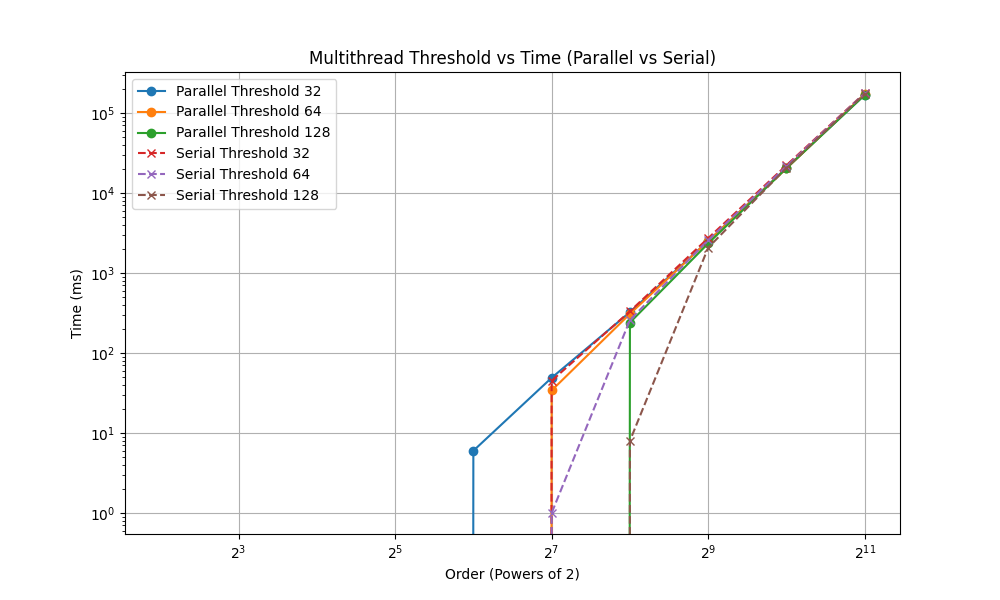
\includegraphics[width=\linewidth]{perf_graph.png}

  \item The running times for both the serial elision and multi-threaded version of the code is stored in \verb|serial_perf.csv| and \verb|parallel_perf.csv|, respectively. The speedup is shown in the graph above. The processor is an Apple M1 Pro chip with 8 cores, 8 threads, a 128-byte cache-line size, 128 KB of L1 cache per core, 24 MB of L2 cache, and 24 MB of L3 cache.
  
  \item For simplicity, we assume Case 1 when analyzing the cache complexity of matrix multiplication as shown in class (indeed, this is justified since experimentally our 2048 * 2048 * 4 byte matrix fits inside our 22 MB cache), which has a cache complexity of $\Theta(n^3/L(\sqrt Z))$. (Note that in our example, the matrices are square so $m = n = p = n$). Writing to the result matrix will also incur cache misses equivalent to $\Theta(n^3/L)$. Using the Master theorem for the recurrence
  
  $$
  Q(n, Z, L) = 2Q(n/2, Z, L) + \Theta(n^3/L(\sqrt Z)) + \Theta(n^3/L)
  $$

  yields a cache complexity of $\Theta(n^3/L)$ for the serial version of the algorithm.

\end{enumerate}

\section*{Problem 2}

\begin{enumerate}
  \item \begin{verbatim}
    (ps is sorted by x-coordinate)
    PointPair closest_pair(Point ps[], int n)
    {
        if (n <= 3) return closest_pair_brute_force(ps, n);
        int mid = n / 2;
        PointPair left = spawn closest_pair(ps, mid);
        PointPair right = closest_pair(ps + mid, n - mid);
        sync;
        PointPair middle = merge(ps, n, left, right);
        return min_distance(left, right, middle);
    }

    PointPair merge(Point ps[], int n, PointPair left, PointPair right)
    {
        min_d = minimum distance of left and right;
        boundary_ps = points within min_d of the middle;
        sort boundary_ps by y-coordinate
        for (i = 0; i < boundary_ps.size(); i++) {
            for (j = i + 1; j < boundary_ps.size() && j < i + 7; j++) {
                if (distance(boundary_ps[i], boundary_ps[j]) < min_d) {
                    min_d = distance(boundary_ps[i], boundary_ps[j]);
                    min_pair = (boundary_ps[i], boundary_ps[j]);
                }
            }
        }
        return min_pair;
    }
  \end{verbatim}

  Each recursive call of \verb|closest_pair| calls \verb|merge| which takes $O(n \log n)$ time to sort the points by their y-coordinate. Since we split the points by 2 on each recursive call, the depth of the recursion tree is at most $\log n$. So the work is $O(n \log^2 n)$ (this can also be shown by the Master theorem).

  \item A multi-threaded version of the above algorithm could \verb|spawn| a child for each recursive call of \verb|closest_pair|. Because the span of the algorithm is $O(n \log n)$ (with an infinite number of processors, a single processor would still need to do $O(n \log n)$ work due to the sort in \verb|merge|), the parallelism would be $O(\frac{n \log^2 n}{n \log n}) = O(\log n)$.
  
  \item Instead of using a standard sorting algorithm in $O(n \log n)$ as in the above, we can use a parallel merge-sort algorithm which takes $O(n)$ time. This would reduce the work to $O(n \log n)$ and the span to $O(\log^2 n)$, resulting in a parallelism of $O(\frac{n}{\log n})$.
  
  Note that the parallel merge-sort algorithm takes $O(n)$ since the merge step can be done in parallel. The work is $O(n \log n)$ since the depth of the recursion tree is $\log n$ and the work done at each level is $O(n)$. The span is $O(\log^2 n)$ since the merge step takes $O(\log n)$ time.
  
  \item The implementation is in \verb|closest_pair.c|. Output is shown in \verb|q2.out| (not using cilk) and \verb|q2_cilk.out| (using cilk). Note that as the number of points increases by a factor of 10, the running time increases by a factor of 100 approximately for the naive implementation. The running time for the cilk implementation increases by a factor of 10 approximately. This is consistent with the parallelism of the cilk implementation being $O(\frac{n}{\log n})$ and the complexity of the naive algorithm being $O(n^2)$. 
\end{enumerate}
\end{document}
